\section{Missbrauch des „Wo ist?“ Dienstes}
\label{sec:Missbrauch}

Das Hauptangriffsziel für Angreifer des „Wo ist?“ Dienstes sind die Standortdaten der Nutzer.
Apple ergreift verschiedene Maßnahmen, um die Sicherheit der Standortdaten sicherzustellen, wie bei der Erläuterung der Funktionsweise in \autoref{sec:Funktionsweise_FindMy} bereits gezeigt wurde.
Dennoch besteht Missbrauchspotenzial, gegen welches der Dienst nicht oder nicht ausreichend geschützt ist, wie unter anderem durch Tonetto \textit{et al.} \cite{Tonetto_FindMy} aufgezeigt werden konnte.
Zunächst werden in \autoref{tab:cia_findmy} die allgemeinen Sicherheitsziele Vertraulichkeit (\textit{Confidentiality}), Integrität (\textit{Integrity}) und Verfügbarkeit (\textit{Availability}) sowie mögliche Angriffsziele im Kontext des „Wo ist?“ Dienstes erklärt.
Darauf aufbauend wird gezeigt, wie die von Apple implementierten Sicherheitsmaßnahmen die Sicherheitsziele in vielen Fällen unterstützen.
Im Anschluss können in \autoref{sec:szenarien} konkrete Missbrauchsszenarien aufgezeigt werden, gegen welche Apple nur unzureichende Maßnahmen ergreift, und welche somit die Sicherheit und Privatsphäre der Nutzer und sogar Dritter gefährden können.

\begin{table}[h]
  \caption{Sicherheitsziele des „Wo ist?“ Dienstes und mögliche Angriffsziele.}
  \label{tab:cia_fincmy}
  \begin{tabularx}{\textwidth}{ |l|X|X| }
    \hline
    \textbf{Sicherheitsziel}  & \textbf{Beschreibung}                                               & \textbf{Angriffsziel}                                           \\
    \Xhline{0.5mm}
    \hline
    Vertraulichkeit           & Standortdaten sind nur befugten Personen zugänglich.                & Standort eines Nutzers oder eines Geräts erhalten.              \\
    \hline
    Integrität                & Standortdaten sind vor Manipulation geschützt.                      & Standortdaten eines Nutzers oder eines Geräts manipulieren.     \\
    \hline
    Verfügbarkeit             & Standortdaten können abgerufen werden.                              & Verhindern, dass Standortdaten abgerufen werden können.         \\
    \hline
  \end{tabularx}
\end{table}

Die von Heinrich \textit{et al.} \cite{Heinrich_FindMy} identifizierten Angreifermodelle in \autoref{fig:adversary_models} zeigen verschiedene Möglichkeiten, wie ein Angreifer versuchen kann, den Dienst anzugreifen.
Sie gehen von vier verschiedenen Angreifermodellen aus, die sich im Angriffsvektor unterscheiden.
Potenzielle Angriffe können demnach von lokal installierten Anwendungen, Geräten in \ac{BLE}-Reichweite, einem klassischen Netzwerkangreifer und dem Dienstanbieter, also von Apple ausgehen.
Für jeden Angriffsvektor werden verschiedene mögliche Ziele definiert.
\begin{figure}[ht]
  \centering
  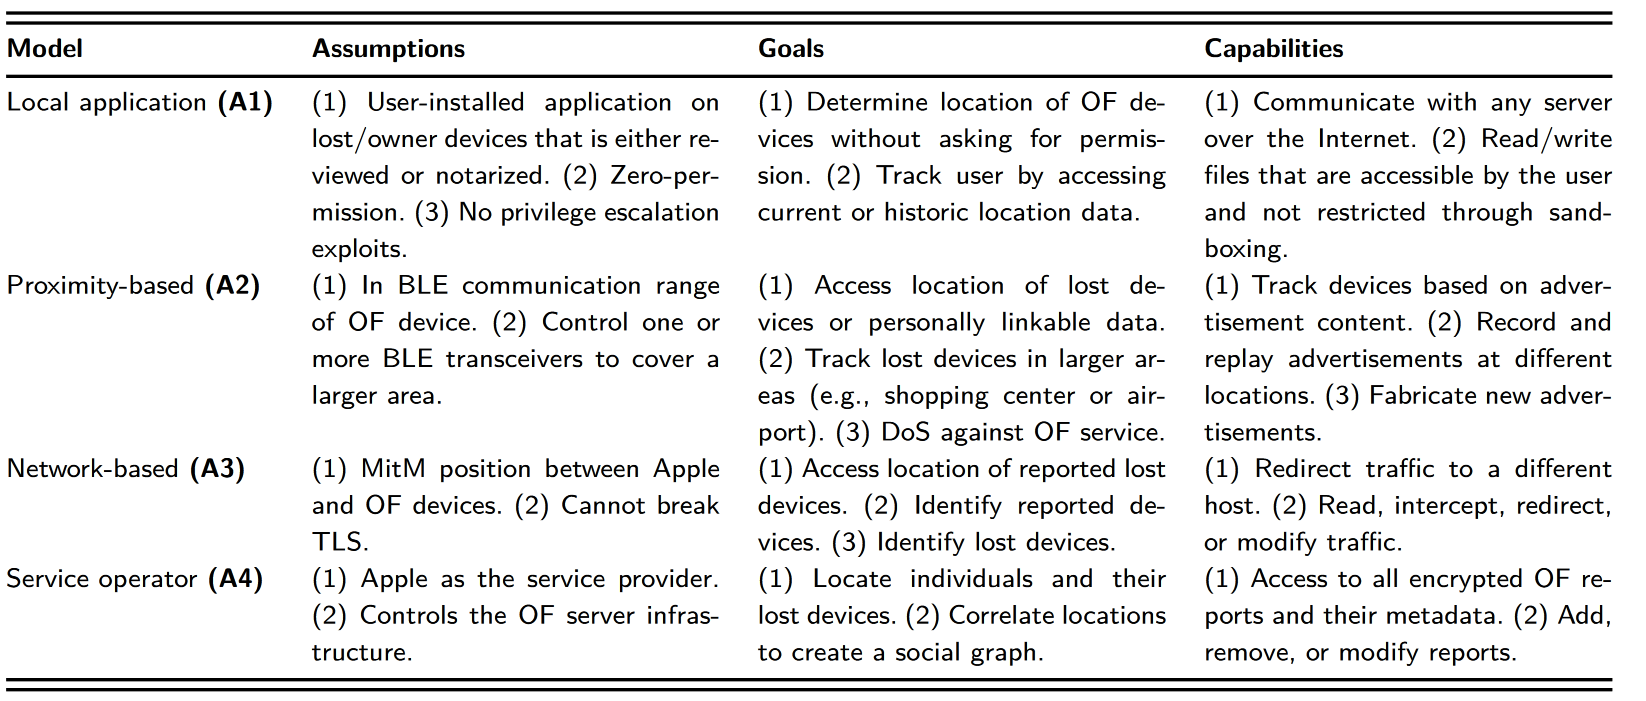
\includegraphics[width=0.9\textwidth]{img/adversary_models}
  \caption{Angreifermodelle für den „Wo ist?“ Dienst \cite{Heinrich_FindMy}.}
  \label{fig:adversary_models}
\end{figure}

\autoref{tab:cia_adversary_models} ordnen den Zielen der einzelnen Angreifermodelle die jeweiligen Sicherheitsziele zu.
\begin{table}[h]
  \caption{Zuordnung der Ziele der Angreifermodelle zu den allgemeinen Sicherheitszielen.}
  \label{tab:cia_adversary_models}
  \centering

  \begin{tabularx}{\textwidth}{ |l|X|X|l|X| }
    \hline
    \textbf{Angreifermodell}  & \textbf{Ziel} & \textbf{Vertraulichkeit} & \textbf{Integrität} & \textbf{Verfügbarkeit} \\
    \Xhline{0.5mm}
    \hline
    \multirow{2}{*}{A1} & (1) & \cmark & & \\
    \cline{2-5}
    & (2) & \cmark & & \\
    \hline
    \multirow{3}{*}{A2} & (1) & \cmark & & \\
    \cline{2-5}
    & (2) & \cmark & & \\
    \cline{2-5}
    & (3) & & & \cmark  \\
    \hline
    \multirow{3}{*}{A3} & (1) & \cmark & & \\
    \cline{2-5}
    & (2) & \cmark & & \\
    \cline{2-5}
    & (3) & \cmark & & \\
    \hline
    \multirow{2}{*}{A1} & (1) & \cmark & & \\
    \cline{2-5}
    & (2) & \cmark & & \\
    \hline
  \end{tabularx}
\end{table}
Dabei fällt auf, dass der Fokus auf der Vertraulichkeit der Daten liegt.
Als personenbezogene Daten unterliegen die Standortdaten der \ac{DSGVO} und sind für Angreifer ein lohnenswertes Ziel.
Durch mögliche Rückschlüsse auf beispielsweise religiöse oder politische Überzeugungen sind Standortdaten nach Artikel 9 \ac{DSGVO} häufig auch als sensible personenbezogene Daten zu betrachten.
Deshalb ist die Vertraulichkeit der Standortdaten besonders schützenswert.
Sollten Angreifer Zugriff auf die Standortdaten erhalten, könnten sie diese für viele verschiedene Zwecke missbrauchen.
Zum Beispiel können diese Daten für gezielte Diskriminierung, Verfolgung und Überwachung durch Dritte oder auch durch staatliche Akteure verwendet werden.
Bei der Werbung für den „Wo ist?“ Dienst \cite{Apple_WoIst} wird der Fokus stark auf die Privatsphäre gelegt und betont, dass selbst Apple keinen Zugriff auf die Daten hat.

Das \textit{Proximity-based} Modell (A2 in \autoref{tab:cia_adversary_models}) zielt auf die Verfügbarkeit der Daten ab.
Wird die Verfügbarkeit beeinträchtigt, ist es für den Besitzer eines Geräts nicht mehr möglich, die aktuellen Standortdaten abzurufen.
Dies kann für einen Angreifer zum Beispiel im Zusammenhang mit dem Diebstahl eines Geräts nützlich sein.

Die Beeinträchtigung der Integrität der Daten wird in \cite{Heinrich_FindMy} nicht als Ziel eines Angreifers untersucht.
Jedoch ist ein gewisser Zusammenhang mit der Verfügbarkeit gegeben.
Durch gezielte Manipulation der Daten kann der Besitzer beispielsweise nicht mehr unterscheiden welche Daten korrekt sind, was die Verfügbarkeit stark beeinträchtigen kann.
Außerdem wird allgemeiner Missbrauch des „Wo ist?“ Dienstes für Zwecke, für welche dieser nicht konzipiert wurde, in \cite{Heinrich_FindMy} nicht explizit betrachtet.
Solche Missbrauchsszenarien werden in \autoref{sec:szenarien} vorgestellt.


\subsection{Auswirkungen der Sicherheitsmaßnahmen}

\subsubsection{Ende-zu-Ende Verschlüsselung}
Die Betrachtung der Funktionsweise in \autoref{sec:Funktionsweise_FindMy} zeigt, wie die Ende-zu-Ende-Verschlüsselung des Dienstes technisch umgesetzt wird.
Durch die Verwendung dieses Verschlüsselungsmechanismus kann unter der Annahme, dass der Angreifer die Verschlüsselung nicht brechen kann, gewährleistet werden, dass nur der Besitzer eines verlorenen Geräts die Standortdaten entschlüsseln kann.
Sollte einem Angreifer gelingen die Daten direkt von Apples Server abzurufen, oder über einen \ac{MITM} Angriff die verschlüsselten Daten zu erhalten, können diese ohne die nur auf den Owner Devices verfügbaren Schlüssel nicht entschlüsselt werden.
Dabei werden ein \ac{MITM}-Angriffe durch die Verwendung von \ac{TLS} mit Certificate Pinning bei der Kommunikation mit Apples Servern verhindert \cite{Heinrich_FindMy}.
Durch die Ende-zu-Ende Verschlüsselung werden alle vom Netzwerkangreifer (A3 in \autoref{fig:adversary_models}) ausgehenden Bedrohungen adressiert.
Die zur Entschlüsselung benötigten Schlüssel werden auf den Geräten des Besitzers in der als sicher geltenden iCloud Keychain gespeichert.
So werden auch die von lokalen Angreifern (A1 in \autoref{fig:adversary_models}) ausgehenden Bedrohungen behandelt.
Eine in \cite{Heinrich_FindMy} aufgedeckte Schwachstelle, die aufgrund von unsicherer Speicherung der Schlüssel unbefugten Zugriff auf die Standortdaten ermöglicht, wurde durch Apple mittlerweile behoben.
Zusätzlich wird es durch die Ende-zu-Ende-Verschlüsselung auch Apple unmöglich gemacht, auf die Standortdaten der Nutzer zuzugreifen, womit das Lokalisieren durch den Dienstanbieter (A4 mit Ziel (1) in \autoref{fig:adversary_models}) verhindert wird.
Außerdem verbessert die Verschlüsselung die Integrität der Daten, da einmal verschlüsselte Daten ohne Entschlüsselung nicht manipuliert werden können, ohne dass diese Manipulation erkannt werden kann.
Jedoch ist es möglich, dass die Standortdaten auf Basis eines Replay-Angriffes generiert wurden.
Auf dieses Szenario wird in \autoref{sec:szenarien} näher eingegangen.


\subsubsection{Schlüsselrotation}
Die Schlüsselrotation der Advertising Keys im Intervall von 15 Minuten bei Endgeräten und bis zu 24 Stunden bei Accesories, wie in \autoref{sec:Funktionsweise_FindMy} beschrieben, trägt ebenfalls zur Vertraulichkeit der Standortdaten bei.
Durch die regelmäßige Rotation der Schlüssel wird das Tracking von Geräten anhand der im Advertising gesendeten Daten erschwert.
Damit richtet sich diese Maßnahme gezielt gegen das Tracking durch einen Angreifer in der Nähe (A2 mit Ziel (2) in \autoref{fig:adversary_models}).
Außerdem müssten für einen solchen Angriff viele scannende Geräte so positioniert werden, dass auch bei Bewegung die Advertisement Pakete des zu verfolgenden Geräts von einem der scanner erfasst wird.
Um größere Bereiche abzudecken, wären jedoch sehr viele scannende Geräte notwendig, was den Angriff bereits deutlich erschwert.
In Verbindung mit der Schlüsselrotation ist die Verfolgung auch mit hohem Aufwand nur für das Intervall der Schlüsselrotation möglich.
Allerdings können AirTags und Drittanbieterprodukte durch das längere Intervall für bis zu 24 Stunden über einen solchen Angriff verfolgt werden.
Für Angreifer ist der Angriff jedoch insgesamt so komplex, dass eine direkte Verfolgung des Opfers in den meisten Fällen praktikabler wäre.
Heinrich \textit{et al.} \cite{Heinrich_FindMy} betrachten die Schlüsselrotation als ausreichend, um die Verfolgung von Geräten nach diesem Muster zu verhindern.
Jedoch zum Zeitpunkt ihrer Analyse keine Geräte mit einem Intervall der Schlüsselrotation von mehr als 15 Minuten auf dem Markt.

% TODO: eventuell mehr der Gegenmaßnahmen nach hinten verschieben und stattdessen mehr auf konkreten Missbrauch eingehen
% eventuell auch die von Apple bereits getroffenen Gegenmaßnahmen mit Bewertung hier und alles andere später
\subsection{Missbrauchsszenarien ohne ausreichende Gegenmaßnahmen}
\label{sec:szenarien}

\subsubsection{Replay-Angriff}
Durch die Ende-zu-Ende-Verschlüsselung und den authentifizierten Upload der Standortdaten kann die Integrität der Standortdaten in vielen Fällen geschützt werden.
Allerdings können über einen Replay-Angriff manipulierte Standortdaten, welche korrekt verschlüsselt sind und authentifiziert hochgeladen werden, auf Apples Server gelangen.
Somit kann die Integrität der abgerufenen Standortdaten nicht mehr gewährleistet werden und die Verfügbarkeit der Standortdaten kann beeinträchtigt werden, da der Nutzer eventuell nicht mehr erkennen kann, welche Daten korrekt sind und somit keine verlässliche Standortinformation erhält \cite{Heinrich_FindMy}.
Dieser Angriff entspricht dem \ac{DOS}-Angriff durch einen Angreifer in der Nähe (A2 mit Ziel (3) in \autoref{fig:adversary_models}).

Um einen solchen Angriff durchzuführen, kann ein Angreifer die Advertisement Pakete eines Gerätes aufzeichnen und an anderen Orten wieder abspielen.
Geräte in der Nähe empfangen die Pakete und senden Standortdaten verschlüsseln und korrekt authentifiziert an Apple.
Der Besitzer kann die manipulierten Standortdaten erhalten und diese eventuell als korrekt interpretieren.
Es ist unklar, ob Apple gegen diese Art der Manipulation Maßnahmen ergreift.
Das Design des Dienstes lässt prinzipiell verschiedene Maßnahmen zu, um den Angriff zumindest zu erkennen.
Die „Wo ist?“ App könnte die Plausibilität der Daten prüfen und unplausible Daten dem Nutzer als eventuell manipuliert anzeigen.
Eine Plausibilitätsprüfung wäre zum Beispiel anhand der Zeitpunkte der Standortdaten möglich.
Große Veränderungen des Standorts in kurzer Zeit könnten auf einen Replay-Angriff hindeuten.
Außerdem könnte das Owner Device bestimmen, welcher Advertising Key zum Zeitpunkt der Generierung des Location Reports aktiv war und so überprüfen ob der Location Report mit dem passenden Advertising Key erstellt wurde, oder ob ein älterer Schlüssel verwendet wurde.
So könnte zumindest der Zeitraum eines Replay-Angriffs auf das Intervall der Schlüsselrotation eingegrenzt werden.

\subsubsection{Angriff auf die Verfügbarkeit durch Angreifer mit physischem Zugriff}
Die Verfügbarkeit der Standortdaten ist für die Betrachtung im Rahmen dieser Arbeit weniger relevant, da das Design des Dienstes vergleichsweise wenige Auswirkungen auf die Verfügbarkeit hat.
Dennoch ist die Verfügbarkeit durch verschiedene Angriffe bedroht.
Zum Beispiel könnte ein direkter \ac{DOS} Angriff auf die Server von Apple erfolgen, was allerdings als unwahrscheinliches Bedrohungsszenario angesehen werden kann.
Relevanter sind hingegen Angriffe auf die Verfügbarkeit der Standortdaten durch physischen Zugriff oder die Nähe des Angreifers zum verlorenen Gerät.
Bei physischem Zugriff, beispielsweise in Zusammenhang mit Diebstahl, kann zum Beispiel durch Zerstörung des Geräts oder durch das Entfernen der Batterie, verhindert werden, dass neue Standortinformationen des Geräts generiert werden.
Die Zerstörung eines Endgeräts bei einem Diebstahl desselben wäre wenig zielführend.
Allerdings ist die Zerstörung eines Trackers, wie eines AirTags, beim Diebstahl des Gegenstandes, an welchem der Tracker befestigt ist, ein wahrscheinliches Szenario.
In diesem Fall würde jedoch auch das Entfernen des Trackers vom gestohlenen Gegenstand oder das Entfernen der Batterie aus dem Tracker ausreichen, um die Nachverfolgbarkeit des Gegenstandes zu verhindern.
Gegen solche Angriffe können keinerlei IT-Security-Maßnahmen ergriffen werden.
Jedoch ließe sich die Auffindbarkeit von Trackern durch selteneres Advertisement verringern, wodurch ein Angreifer mehr Zeit benötigen würde, um den Tracker zu finden.
Diese Maßnahme würde allerdings gleichzeitig das Tracking anderer Personen unter Verwendung eines versteckten Trackers erleichtern.
Generell ist der „Wo ist?“ Dienst nicht als Hilfsmittel gegen Diebstahl konzipiert und wird auch nicht als solches beworben \cite{Apple_WoIst}.

\subsubsection{Angriff auf die Verfügbarkeit durch nahe Angreifer}
Bei dem von Garg \textit{et al.} \cite{Garg_Secure_Tracker} als sicher vorgeschlagenen Systemen ist neben dem Entfernen der Batterie auch das gezielte Entladen dieser ohne physischen Zugriff möglich.
Dieses System ist so gestaltet, dass der aktuelle Standort vom Finder Device an das Lost Device gesendet wird, welches die Daten verschlüsselt zurückgibt.
In diesem Szenario kann ein Angreifer durch häufiges senden von Standorten an das Lost Device unter Zuhilfenahme der energieintensiven Verschlüsselungsoperationen, die Batterie des Lost Devices entladen.
Insbesondere für Accessories geringer Batteriekapazität ist dies ein relevantes Bedrohungsszenario.
Da bei Apples System die Verschlüsselung nicht auf dem verlorenen Gerät, sondern auf dem Finder Device erfolgt, ist ein solcher Angriff vermutlich schwieriger.
Dennoch besteht ein gewisses Potenzial, da zumindest Accesories \ac{BLE}-Verbindungen zulassen, um zum Beispiel einen Ton abzuspielen, was ebenfalls genutzt werden könnte, um die Batterie zu entladen \cite{Heinrich_AirGuard}.

\subsubsection{Direktes Tracking von Personen}
Das Szenario des direkten Tracking von Personen bezieht sich auf die Verfolgung durch AirTags oder andere kleine Tracker.
Durch die kleine Größe der Tracker können diese in Jacken, Rucksäcken oder an Fahrzeugen befestigt werden, um einzelne Personen gezielt zu verfolgen.
Dieser Angriff wurde bereits vielfach in der Praxis beobachtet und für Stalking oder Autodiebstahl genutzt \cite{NYT_Airtags}.
Der „Wo ist?“ Dienst bietet zwar eine Funktion zur „Unwanted tracking detection“, um Nutzer auf mögliche Verfolgung hinzuweisen \cite{Apple_FindMySpec}.
Allerdings wurde bereits gezeigt, dass diese Funktion leicht umgangen werden kann \cite{Mayberry_Tracking} und in vielen Fällen nicht zuverlässig vor Tracking warnen kann \cite{Heinrich_AirGuard}.
Darüber hinaus ist die Funktion nur für iOS-Geräte direkt verfügbar, sodass für Android-Nutzer keinerlei Warnung erfolgt.
Demnach ist dieses Szenario durchaus ein Szenario ohne ausreichende Gegenmaßnahmen.
Inzwischen bietet Apple eine App für Android an, um die Warnung vor Tracking auch für Android-Nutzer zu ermöglichen, welche jedoch von Heinrich \textit{et al.} \cite{Heinrich_AirGuard} mangels Features nicht als ausreichend angesehen wird.
Die Drittanbieter-App \textit{AirGuard} für Android bietet eine ähnliche Warnfunktion, welche in Tests besser abschneidet als die Warnfunktion von iOS \cite{Heinrich_AirGuard}.
Insbesondere erkennt nur AirGuard das Tracking durch inoffizielle Tracker.
Solche Tracker, die das „Wo ist?“ Netzwerk ohne explizite Erlaubnis von Apple nutzen, können von Angreifern leicht aus kostengünstiger \ac{BLE}-Hardware und Open-Source Software selbst gebaut werden.
Diese können die von Mayberry \textit{et al.} \cite{Mayberry_Tracking} vorgestellten Maßnahmen nutzen, um die offizielle Unwanted tracking detection zu umgehen.
Inoffizielle Tracker, welche ein Intervall von weniger als einer Stunde für die Schlüsselrotation verwenden, können allerdings weder von der offiziellen Warnfunktion noch von AirGuard erkannt werden \cite{Heinrich_AirGuard}.


\subsubsection{Indirektes Tracking von Personen}
Beim indirekten Tracking werden Personen nicht durch Tracker direkt verfolgt.
Stattdessen werden anhand der Uploadzeitpunkte von Location Reports Rückschlüsse auf die Bewegung von Personen gezogen.
Dieses Missbrauchsszenario wurde von Tonetto \textit{et al.} \cite{Tonetto_FindMy} vorgestellt und kann nicht nur für das schadhafte Tracking von Personen genutzt werden, sondern auch als privatsphärefreundliche Funktion zum Crowd-Monitoring.
Da Finder Devices Location Reports generell gebündelt hochladen, und Apples Server die Uploadzeitpunkte mit einer Genauigkeit von wenigen Millisekunden speichern, ist es für möglich, Location Reports, die vom gleichen Gerät stammen, anhand der Uploadzeitpunkte zu identifizieren \cite{Tonetto_FindMy}.
Während Finder Devices mit Mobilfunkverbindung Location Reports in der Regel erst nach einigen Stunden hochladen, erfolgt der Upload bei einer \ac{WLAN}-Verbindung deutlich schneller.
Wechselt ein Finder Device von einer Mobilfunkverbindung zu einer \ac{WLAN}-Verbindung werden die zwischengespeicherten Location Reports in der Regel kurz darauf hochgeladen.
Unter der Annahme, dass Personen außerhalb einiger weniger Orte, wie zum Beispiel der eigenen Wohnung, nicht dauerhaft mit einem \ac{WLAN}-Netzwerk verbunden sind, werden außerhalb dieser Orte erstellte Location Reports in etwa zur gleichen Zeit hochgeladen \cite{Tonetto_FindMy}.

Platziert ein Angreifer mehrere Tracker an verschiedenen Orten, erfassen Finder Devices diese und generieren jeweils Location Reports.
Jeder dieser Location Reports gibt an, zu welchem Zeitpunkt das Finder Device an welcher Position war.
Werden diese Location Reports gebündelt hochgeladen, kann der Angreifer die zusammengehörigen Location Reports anhand der Uploadzeitpunkte identifizieren.
Aus den Positionen und Zeitpunkten der Erstellung der Reports kann die Bewegung des Finder Device rekonstruiert werden \cite{Tonetto_FindMy}.


Zum privatsphärefreundlichen Crowd-Monitoring werden einzelne Tracker an öffentlichen Orten platziert.
Finder Devices, die sich in der Nähe dieser Tracker befinden, generieren Location Reports.
Diese Reports können von Apples Servern heruntergeladen werden und erlauben über die Anzahl der Reports Rückschlüsse auf die Anzahl der Personen, die sich in der Nähe des Trackers aufgehalten haben.
Über die Verwendung mehrere Tracker lassen sich auch die Bewegungen von Menschenmassen rekonstruieren.
Dieser Missbrauch des „Wo ist?“ Dienstes kann als Alternative zu aktuellen Bilderkennungs-basierten Crowd-Monitoring-Systemen verwendet werden und erlaubt eine ähnliche Genauigkeit.
Zusätzlich ist dieser Ansatz privatsphärefreundlicher als die Bilderkennung, da keine personenbezogenen Daten erhoben werden \cite{Tonetto_FindMy}.



% Konkrete Szenarien:
% - Tracking von Personen
%   - Indirekt: wie von Tonetto et al. gezeigt -> über Tracker in der Umgebung, weniger genau
% - Verdeckter Datentransfer
%   - wie von Tonetto et al. und bei SendMy gezeigt
% - Korrelation der Positionen durch Apple, eher theoretisch
